\documentclass[conference]{IEEEtran}
\IEEEoverridecommandlockouts

\usepackage{cite}
\usepackage{amsmath,amssymb,amsfonts}
\usepackage{graphicx}
\usepackage{xcolor}
\usepackage{float}
\usepackage{url}

\begin{document}

\title{Sincronizacion de procesos en sistemas operativos}

\author{
\IEEEauthorblockN{Juan Sebastian Rodriguez Carreño}
\IEEEauthorblockA{20231020107}
}

\maketitle

\begin{abstract}
This work presents a multithreaded simulation of water consumption from a shared jug to study process synchronization in operating systems. A set of threads competing for a common resource is modeled, and the critical section is protected through mutual exclusion mechanisms. The development allows identifying race conditions, comparing synchronization alternatives, and reasoning about shared-state consistency during concurrent execution.
\end{abstract}

\begin{IEEEkeywords}
synchronization, threads, critical section, mutual exclusion, race condition
\end{IEEEkeywords}

\section{Introduccion}
En programacion concurrente, varios hilos pueden acceder de forma simultanea a un mismo recurso, lo que incrementa el rendimiento pero tambien introduce riesgos de inconsistencia. Cuando dos o mas hilos leen y escriben una variable compartida sin coordinacion, aparece el problema de condicion de carrera, donde el resultado depende del orden de ejecucion.

El escenario de estudio plantea que varias personas beben de una jarra de agua comun. Aunque el problema es simple, contiene los elementos esenciales de sincronizacion: recurso compartido, seccion critica y competencia entre hilos. A partir de este contexto, se implementa una solucion en Python con threading, tomando como base el codigo propuesto y desarrollando los requisitos funcionales del ejercicio.

El objetivo del informe es documentar el analisis del codigo, la modificacion del mecanismo de sincronizacion, la extension con un hilo de reabastecimiento y una discusion tecnica sobre el comportamiento del sistema con y sin proteccion concurrente.

\section{Análisis del código}
El programa parte de una condicion tipica de concurrencia: varios hilos consumidores comparten una unica variable de estado, agua\_disponible. Esta variable representa el nivel real del recurso y, por tanto, cualquier lectura o escritura concurrente sin control puede introducir resultados invalidos.

La evidencia de una ejecucion valida se presenta en la Figura~\ref{fig:ejecucion}, donde se observa la secuencia de consumos por diferentes hilos y la actualizacion consistente del recurso compartido hasta llegar al nivel final de agua.

\begin{figure}[H]
	\centering
	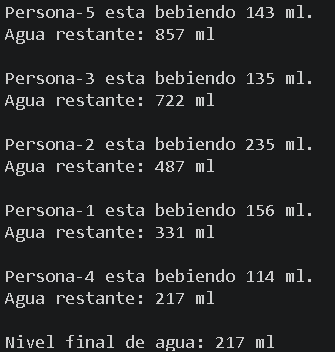
\includegraphics[width=0.72\columnwidth]{Ejecucion.png}
	\caption{Salida de ejecucion del programa con consumos concurrentes y nivel final de agua.}
	\label{fig:ejecucion}
\end{figure}

La seccion critica corresponde al tramo donde se evalua la disponibilidad y se actualiza el saldo. Desde el punto de vista logico, esas dos operaciones deben ejecutarse como una unidad indivisible. Si se separan, un hilo puede validar con un valor antiguo y otro hilo descontar primero, generando una decision basada en un estado que ya cambio.

Esta necesidad justifica el uso de exclusion mutua: no se busca solo ordenar hilos, sino preservar la invariancia del sistema. La regla de invariancia es que el nivel de agua nunca debe ser negativo y que cada consumo aprobado debe corresponder a agua realmente existente. Proteger la seccion critica garantiza esa propiedad en cada iteracion de la simulacion.

Adicionalmente, la llegada aleatoria de los hilos fortalece el analisis porque introduce intercalamientos no deterministas. Esta variabilidad justifica el enfoque sincronizado: no basta con que el programa funcione en una corrida, debe conservar consistencia bajo multiples ordenes de ejecucion.

\section{Modificación del código}
La modificacion propuesta cambia el mecanismo de exclusion mutua de candado a semaforo binario. En la implementacion, esto equivale a inicializar un semaforo con capacidad de una entrada simultanea. La decision se justifica porque mantiene el comportamiento correcto actual y, al mismo tiempo, abre una ruta de escalamiento para escenarios donde se permita mas de una operacion concurrente controlada.

La estructura principal de la simulacion se muestra en la Figura~\ref{fig:flujo-principal}. Alli se evidencia la creacion del recurso compartido, el lanzamiento de hilos consumidores y la espera de finalizacion mediante join, pasos que enmarcan el comportamiento concurrente analizado en este informe.

\begin{figure}[H]
	\centering
	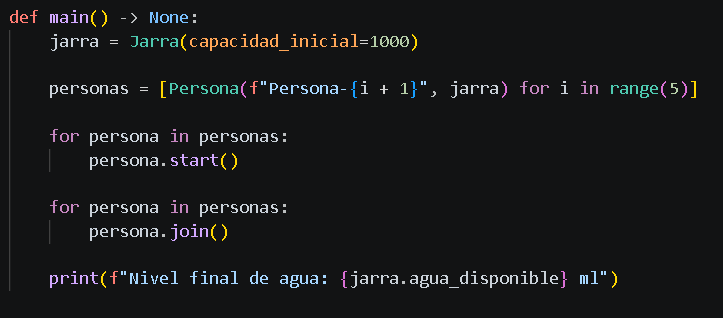
\includegraphics[width=0.95\columnwidth]{flujoPrincipal.png}
	\caption{Flujo principal de la simulacion: inicializacion, inicio y sincronizacion de hilos.}
	\label{fig:flujo-principal}
\end{figure}

Desde el punto de vista funcional, el cambio no altera las reglas del problema: la validacion y el descuento siguen ejecutandose de manera exclusiva. Por esa razon, la consistencia de agua\_disponible se preserva igual que antes. La diferencia relevante es conceptual y de diseno: el semaforo modela explicitamente una cantidad de permisos, mientras que el candado modela un acceso unico sin nocion de cupo.

La justificacion principal de esta modificacion es pedagogica y tecnica. Pedagogica, porque permite contrastar dos primitivas que resuelven el mismo riesgo inmediato; tecnica, porque deja el sistema preparado para futuras extensiones donde el numero de accesos permitidos pueda ajustarse sin redisenar toda la estructura de control.

\section{Extensión del código}
La extension incorpora un hilo de recarga que actua cuando el nivel cae por debajo de un umbral definido. Esta adicion transforma la simulacion en un esquema basico de productor-consumidor, donde unos hilos reducen el recurso y otro hilo lo repone.

La justificacion de esta extension es que permite evaluar sincronizacion en operaciones de signo opuesto sobre el mismo estado compartido. En el escenario inicial solo habia decrementos; con la recarga, ahora coexisten decrementos e incrementos, lo que aproxima mejor el comportamiento de sistemas reales con demanda y reposicion.

Para que la extension sea correcta, tanto el consumo como la recarga deben usar el mismo mecanismo de exclusión mutua. Si solo se protegiera una de las dos operaciones, reapareceria el riesgo de inconsistencia por escrituras intercaladas. Por eso, la decision de reutilizar la misma primitiva en ambos flujos no es opcional, sino una condicion de correccion.

Ademas, incorporar un limite maximo de capacidad se justifica por integridad del modelo: evita sobrellenado y mantiene una segunda invariancia del sistema, donde el nivel de agua permanece dentro del intervalo valido entre cero y la capacidad definida.

\section{Discusión}
Sin sincronizacion, el sistema queda expuesto a decisiones concurrentes sobre informacion obsoleta. Dos hilos pueden validar disponibilidad al mismo tiempo y ambos aprobar consumo, aunque el recurso solo alcanzaba para uno. El efecto observable puede ser saldo negativo, rechazos tardios o reportes de estado contradictorios.

Este fenomeno evidencia una condicion de carrera: la salida final depende del intercalamiento de instrucciones y no de la logica esperada del problema. La justificacion para considerarlo un error critico es que rompe propiedades basicas del modelo, por ejemplo que el recurso no se consume por encima de su capacidad real.

Con sincronizacion, la ejecucion deja de depender del azar del planificador en el tramo critico. La exclusion mutua no elimina el paralelismo global del programa, pero si serializa el acceso al estado compartido donde existe riesgo. Esta combinacion se justifica porque conserva concurrencia en tareas independientes y aplica control estricto solo donde es necesario.

En terminos de costo-beneficio, el pequeno incremento en espera entre hilos se compensa con una mejora clara en confiabilidad. Para sistemas concurrentes orientados a consistencia, esa relacion justifica plenamente la adopcion de primitivas de sincronizacion desde el diseno inicial.

\section{Conclusion}
La simulacion desarrollada demuestra que la sincronizacion no es opcional cuando se manipula estado compartido entre hilos. El uso de exclusion mutua evita que las operaciones de lectura y actualizacion de agua\_disponible se intercalen de forma insegura, preservando la coherencia del sistema.

Adicionalmente, la modificacion a semaforo y la propuesta de reabastecimiento muestran que el problema puede evolucionar hacia modelos mas completos de coordinacion entre productores y consumidores. En conjunto, el ejercicio cumple su proposito pedagogico: evidenciar de manera practica como las primitivas de sincronizacion resuelven errores de concurrencia y permiten construir programas multihilo correctos.

\begin{thebibliography}{00}

\bibitem{b1} A. Silberschatz, G. Gagne y P. B. Galvin, ``Operating System Concepts'', 7ma ed., 2009; 9na ed., 2012; 10ma ed., 2018.

\bibitem{b2} W. Stallings, ``Operating Systems: Internals and Design Principles'', Prentice Hall, 7ma ed., 2011; 8va ed., 2014; 9na ed., 2018.

\bibitem{b3} A. Tanenbaum, ``Modern Operating Systems'', Addison-Wesley, 3ra ed., 2008; 4ta ed., 2014.

\end{thebibliography}

\end{document}
